\section{Operating Basics}

\subsection{Prepare your AXIOM Beta for use}

\begin{center}
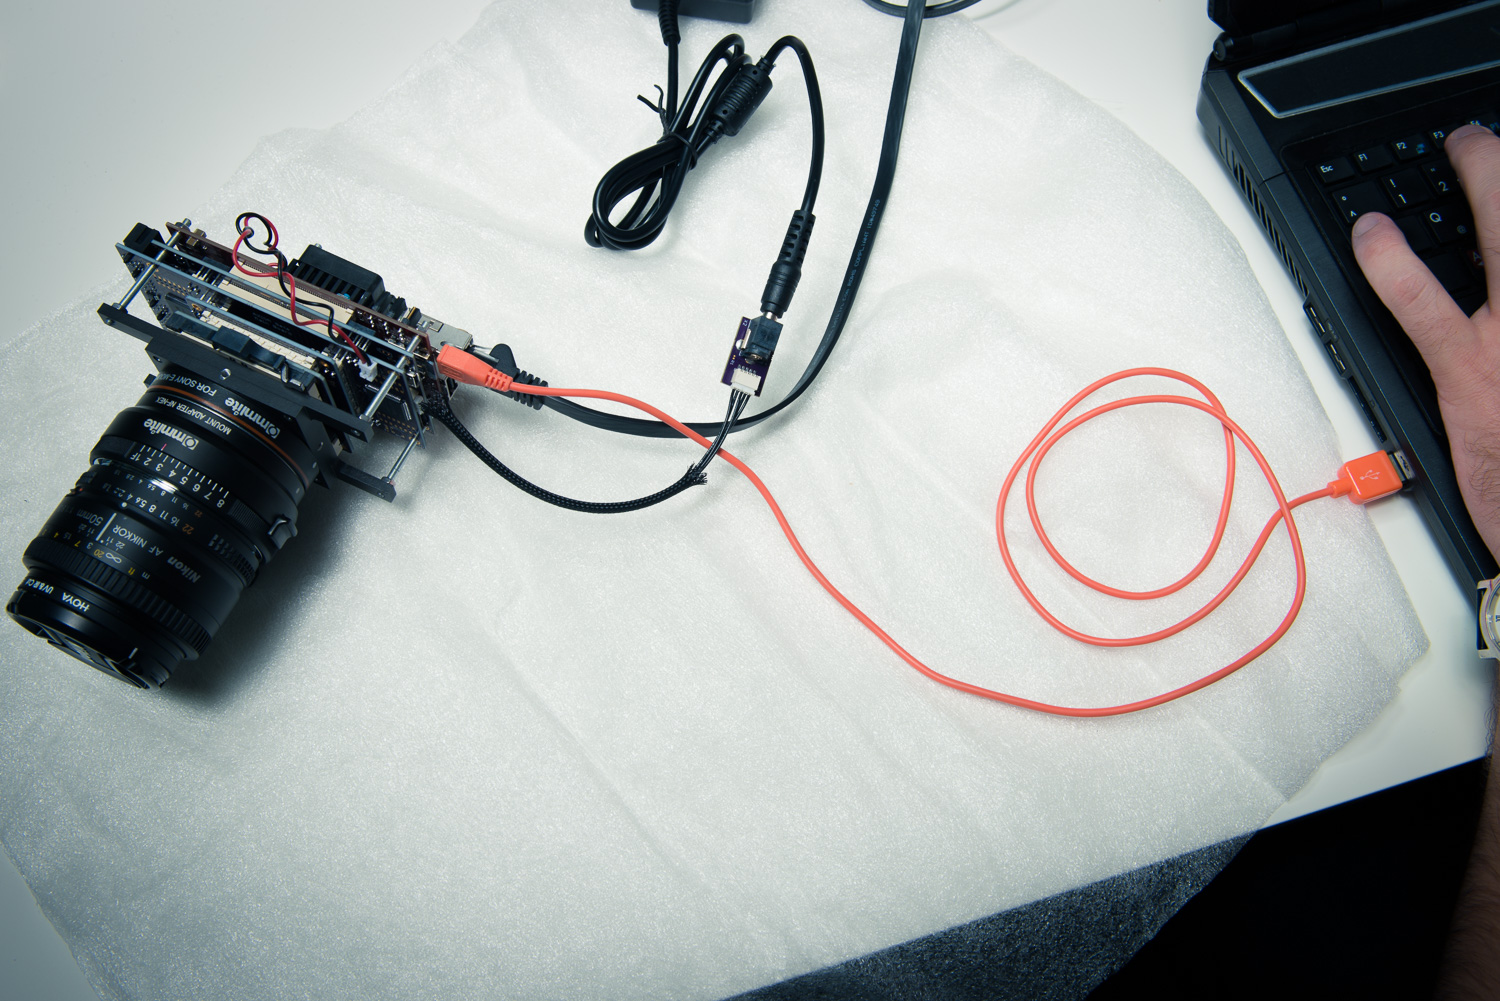
\includegraphics[height=11cm]{images/Getting_Started}\\
\end{center}

1. Use a micro-USB cable to connect the camera's MicroZed development board (USB UART) to a computer. The MicroZed board is the backmost, red PCB. (There is another micro-USB socket on the Power Board, but that is the JTAG Interface.)\\

2. Connect the ethernet port on the MicroZed to an ethernet port on your computer. You might have to use an ethernet adapter on newer, smaller machines which come without a native ethernet port.\\ 

3. Connect the AC adapter to the camera's Power Board. (The power cord plugs into an adapter that connects to the Power Board; to power the camera off at a later point, you need not disconnect the adapter from the board but can just unplug the cord from the adapter.)


\begin{center}
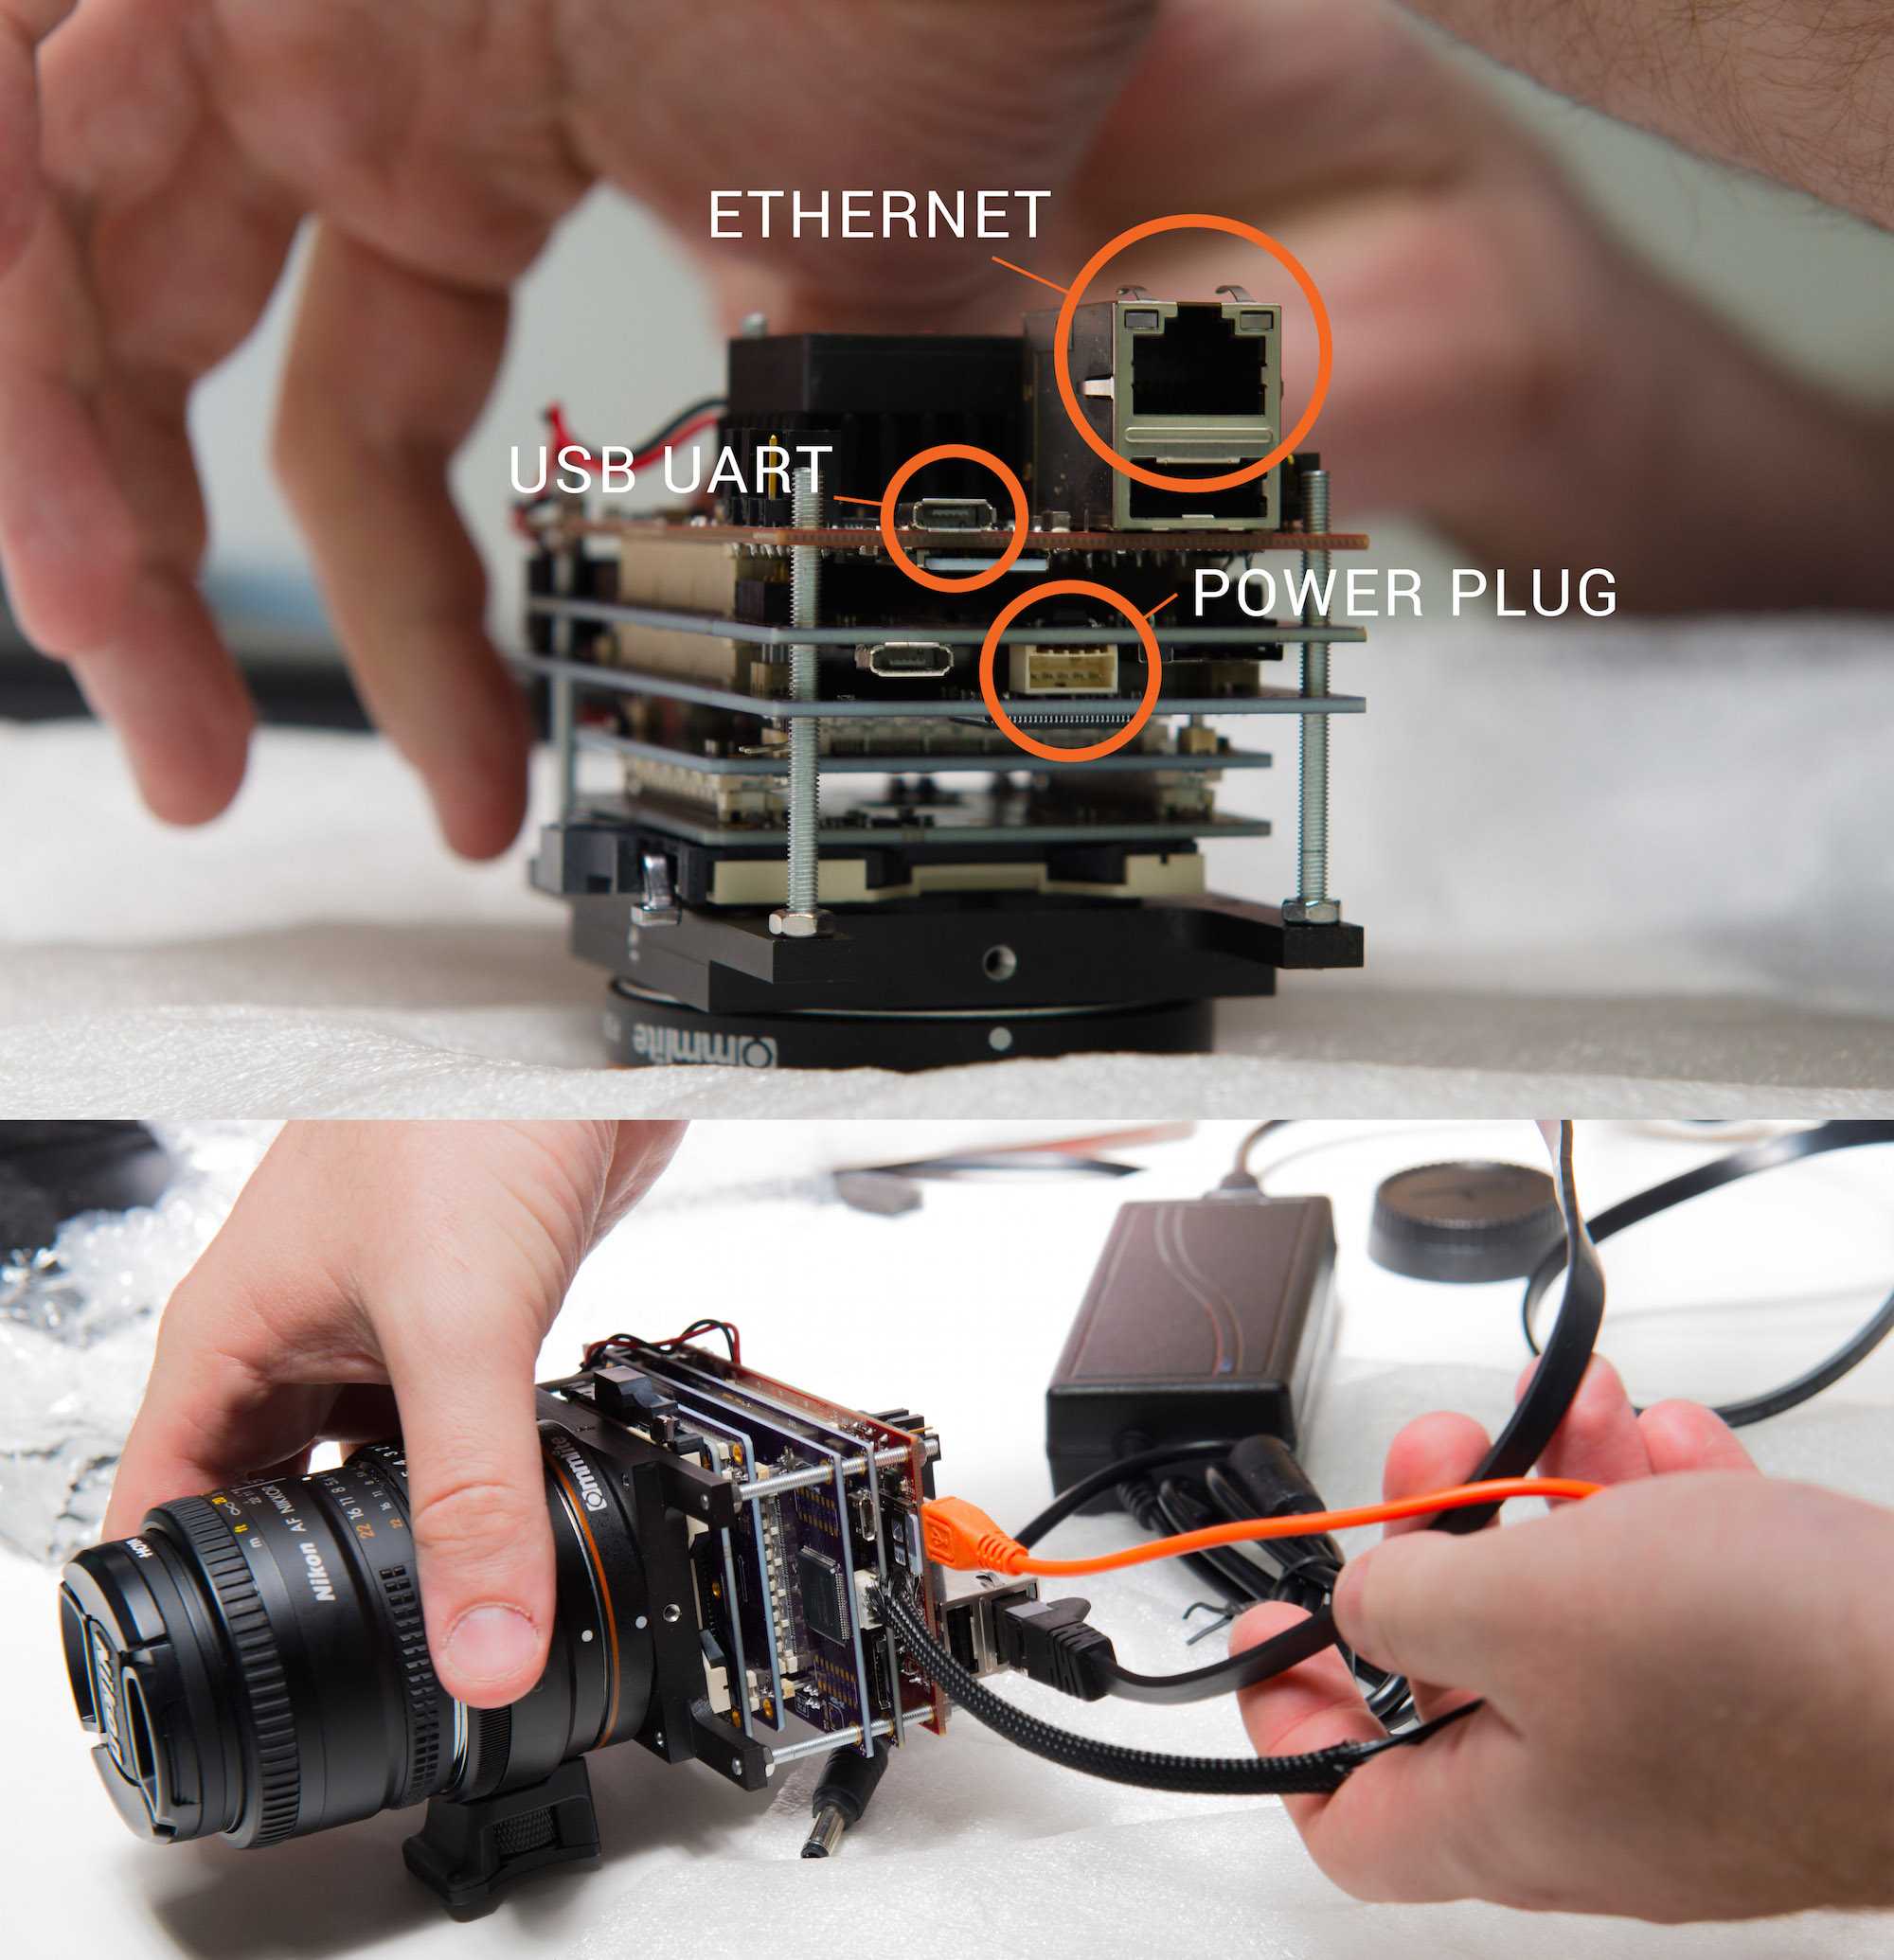
\includegraphics[height=17cm]{images/BetaGuide}\\
\end{center}



\subsection{Prepare your computer for use with AXIOM Beta}

\textbf{Overview -} To communicate with your AXIOM Beta camera, you will send it instructions via your computer's command line.\\

In case you have not worked with a shell (console, terminal) much or ever before, we have prepared detailed instructions to help you get you set up. The steps which need to 	be taken to prepare your machine sometimes differ between operating systems, so pick the ones that are applicable to you(r system). \\

\textbf{Note:} Dollar signs placed in front of commands are not meant to be typed in but denote the command line prompt (a signal indicating the computer is ready for user input). It is used in documentation to differentiate between commands and output resulting from commands. The prompt might look different on your machine (e.g. an angled bracket >) and be preceded by your user name, computer name or the name of the directory which you are currently inside.



\subsubsection{USB to UART Drivers}

For the USB connection to work, you will need drivers for bridging USB to UART (USB to serial). (Under Linux this works out of the box in most 	distributions) for other operating systems they can be \href{https://www.silabs.com/products/development-tools/software/usb-to-uart-bridge-vcp-drivers}{downloaded} from e.g. Silicon Labs' website – pick the software provided for your OS and install it. \\



\subsubsection{Serial Console}

The tool we recommend for connecting to the AXIOM Beta camera via serial port with Mac OS X or Linux is \href{https://linux.die.net/man/1/minicom}{minicom}; for connections from Windows machines, we have used \href{http://www.putty.org/}{Putty}.



\paragraph{Linux Setup}

Check if you already have minicom installed on your system by trying to run it:

\begin{lstlisting}[language=bash,morekeywords=$,keywordstyle=\bfseries,frame=none,xleftmargin=.25in,belowskip=2em, aboveskip=2em]
$ minicom
\end{lstlisting}

Your system will respond with a message like \importantKeyword{bash: command not found: minicom} if it's not installed.\\

\textbf{Install minicom}\\

Install the minicom package like you'd install other software on your system – which could be via a GUI tool or using \importantKeyword{aptitude} or \importantKeyword{apt-get} (for wich you might need super user rights), e.g.: 

\begin{lstlisting}[language=bash,morekeywords=$,keywordstyle=\bfseries,frame=none,xleftmargin=.25in,belowskip=2em, aboveskip=2em]
$ apt-get install minicom
\end{lstlisting}

or

\begin{lstlisting}[language=bash,morekeywords=$,keywordstyle=\bfseries,frame=none,xleftmargin=.25in,belowskip=2em, aboveskip=2em]
$ sudo apt-get install minicom
\end{lstlisting}



\paragraph{MAC OSX Setup}

You will want to have \href{https://brew.sh/}{Homebrew} installed on your system to use \importantKeyword{minicom} for serial communication as it is more convenient than using \importantKeyword{screen}.\\

\textbf{Note:} Homebrew is a package manager for Mac, a piece of software that helps you install other software on your Mac machine, particularly software which is readily available on Linux but which does not come in the form of Mac "applications", which you can download via your web browser and simply drop into your Applications folder.\\ 

Open Terminal.app (or your preferred terminal emulator if you have another installed). Terminal can be found via e.g. Spotlight search or via the Finder menu: \importantKeyword{Go > Utilities > Terminal.app}.\\

Check if you already have brew installed by entering the brew command: 

\begin{lstlisting}[language=bash,morekeywords=$,keywordstyle=\bfseries,frame=none,xleftmargin=.25in,belowskip=2em, aboveskip=2em]
$ brew
\end{lstlisting}

If you don't have Homebrew installed, your shell will reply with something like \importantKeyword{bash: command not found: brew}. Otherwise, it will spit out a list of \importantKeyword{brew} commands.\\ 

\textbf{Install Homebrew}\\

To install Homebrew, go to the \href{https://brew.sh/}{Homebrew} website and follow the install instructions there. You can simply copy the command used for installing Homebrew from their website and paste it into your terminal.\\

\textbf{Install minicom}\\

With brew installed, you want to install minicom:

\begin{lstlisting}[language=bash,morekeywords=$,keywordstyle=\bfseries,frame=none,xleftmargin=.25in,belowskip=2em, aboveskip=2em]
$ brew install minicom
\end{lstlisting}

Homebrew will tell you if you already have minicom installed on your system (e.g. \importantKeyword{Warning: minicom-2.7 already installed}), otherwise it will install it for you. 



\paragraph{Minicom Configuration}

Once you have minicom installed, you need to configure it in order to talk to the camera.\\

You can either use the configuration file we prepared or configure it yourself, following our step-by-step instructions. \\

\textbf{Use Settings File}\\

\textbf{Linux}\\

Go to the minicom setup page:

\begin{lstlisting}[language=bash,morekeywords=$,keywordstyle=\bfseries,frame=none,xleftmargin=.25in,belowskip=2em, aboveskip=2em]
$ minicom -s
\end{lstlisting}

In the "Serial port setup" subpage, check that "Serial Device" 's name is the good one (usually /dev/ttyUSB0 on Linux) and check the baud rate (115200).\\

\textbf{Mac}\\

Download the \href{https://wiki.apertus.org/images/0/06/Minirc.USB0_Mac.zip}{Settings File} for Mac, unzip it and place it in the \importantKeyword{etc} directory of your minicom install.

The minicom installation can be found in the standard directory used by homebrew, \importantKeyword{/usr/local/Cellar}, in a subdirectory based on the minicom version number, e.g. \importantKeyword{/usr/local/Cellar/minicom/2.7/etc}.\\

You can also use Homebrew's \importantKeyword{info} command to find minicom on your hard disk: 

\begin{lstlisting}[language=bash,morekeywords=$,keywordstyle=\bfseries,frame=none,xleftmargin=.25in,belowskip=2em, aboveskip=2em]
$ brew info minicom
\end{lstlisting}

... which will output general information on the installed package, including its install directory e.g.: 

\begin{lstlisting}[breaklines=true, breakatwhitespace=true]
    minicom: stable 2.7 (bottled)
    Menu-driven communications program
    https://alioth.debian.org/projects/minicom/
    /usr/local/Cellar/minicom/2.7 (17 files, 346.6K) *
      Poured from bottle on ...
\end{lstlisting}



\subsubsection{Serial connection (via USB)}

While the AXIOM Beta can be connected to via USB UART (USB to serial), a serial connection is not the preferred way to communicate with the camera but rather in place for monitoring purposes.\\

However, a serial connection is needed to set up communication via ethernet/LAN (the better suited way to talk to the camera): as the Beta only allows for secure ethernet connections, you will have to connect to the camera via serial port first and copy over your SSH key.\\

Below are two different methods for connecting to the AXIOM Beta camera, using a program called minicom and an alternative program called screen. We suggest you try them in the order below, so if you can connect with minicom great, if not try screen. \\



\paragraph{Connect using Minicom}\mbox{}\\

\textbf{Note :} You will not be able to use the terminal window you initiate the serial connection in for anything else (it needs to remain open while you access the camera), so it might make sense to open a separate window just for this purpose.\\

With minicom installed and properly configured, all you need to do is run the following command to start it with the correct settings:

\begin{lstlisting}[language=bash,morekeywords=$,keywordstyle=\bfseries,frame=none,xleftmargin=.25in,belowskip=2em, aboveskip=2em]
$ minicom -8 USB0
\end{lstlisting}

On successful connection, you will be prompted to enter user credentials (which are needed to log into the camera).\\

If your terminal remains blank except for the minicom welcome screen/information about your connection settings, try pressing enter. If this still does not result in the prompt for user credentials – while testing, we discovered the initial connection with minicom does not always work – disconnect the camera from the power adapter, then reconnect it: in your minicom window you should now see the camera's operating system booting up, followed by the login prompt. (From then on, connecting with minicom should work smoothly and at most require you to press enter to make the login prompt appear.)\\

The default credentials are: 

\begin{lstlisting}[language=bash,morekeywords=$,keywordstyle=\bfseries,frame=none,xleftmargin=.25in,belowskip=2em, aboveskip=2em]
    user: root
    password: beta
\end{lstlisting}

\textbf{Alternative tools for serial connection}\\

Before you can use any tool to initiate a serial connection with your Beta camera, you need to know through which special device file it can be accessed.\\

Once the Beta is connected and powered on (and you installed the necessary drivers), it gets listed as a USB device in the \importantKeyword{/dev} directory of your file system, e.g.\\

\importantKeyword{/dev/ttyUSB0} (on Linux)

or

\importantKeyword{/dev/cu.SLAB\_USBtoUART}\\

\importantKeyword{/dev/tty.SLAB\_USBtoUART} (on Mac).

You can use a command such as: 

\begin{lstlisting}[language=bash,morekeywords=$,keywordstyle=\bfseries,frame=none,xleftmargin=.25in,belowskip=2em, aboveskip=2em]
$ ls -al /dev | grep -i usb
\end{lstlisting}

... to list all USB devices currently connected to your machine. 



\paragraph{Connect using Screen}\mbox{}\\

To connect to the camera, use the command: 

\begin{lstlisting}[language=bash,morekeywords=$,keywordstyle=\bfseries,frame=none,xleftmargin=.25in,belowskip=2em, aboveskip=2em]
$ screen file_path 115200
\end{lstlisting}

... where \importantKeyword{file\_path} is the full path to the special device file (e.g. \importantKeyword{/dev/ttyUSB0} or \importantKeyword{/dev/cu.SLAB\_USBtoUART}).

You might have to run the command with superuser rights, i.e.: 

\begin{lstlisting}[language=bash,morekeywords=$,keywordstyle=\bfseries,frame=none,xleftmargin=.25in,belowskip=2em, aboveskip=2em]
$ sudo screen file_path 115200
\end{lstlisting}

On successful connection, you will be prompted to enter user credentials needed for logging into the camera.
If your terminal remains blank, try pressing enter.\\

The default credentials are: 

\begin{lstlisting}[language=bash,morekeywords=$,keywordstyle=\bfseries,frame=none,xleftmargin=.25in,belowskip=2em, aboveskip=2em]
    user: root
    password: beta
\end{lstlisting}



\paragraph{Disconnect}\mbox{}\\

To exit the camera's operating system, use: 

\begin{lstlisting}[language=bash,morekeywords=$,keywordstyle=\bfseries,frame=none,xleftmargin=.25in,belowskip=2em, aboveskip=2em]
$ exit
\end{lstlisting}

The result will be a logout message followed by a new login prompt.

To suspend or quit your \importantKeyword{screen} session (and return to your regular terminal window) use one of the following commands: 

\begin{lstlisting}[language=bash,morekeywords=$,keywordstyle=\bfseries,frame=none,xleftmargin=.25in,belowskip=2em, aboveskip=2em]
CTRL+a CTRL+z
\end{lstlisting}

\begin{lstlisting}[language=bash,morekeywords=$,keywordstyle=\bfseries,frame=none,xleftmargin=.25in,belowskip=2em, aboveskip=2em]
CTRL+a CTRL+\
\end{lstlisting}



\subsubsection{Ethernet connection (using SSH)}

To access the AXIOM Beta via Ethernet (the preferred way to communicate with it and a method which will also work remotely ie. from a machine which is not directly connected to the camera) authentication via SSH is required.\\
 
 

\paragraph{SSH Keys how-to for Linux and Mac}



\subparagraph{Storage location/Find existing keys}

By default, the ssh directory is located at \importantKeyword{~/.ssh}, and contains key files called \importantKeyword{id\_rsa} and \importantKeyword{id\_rsa.pub}, respectively. Check if the directory exists and already contains keys by listing its contents: 

\begin{lstlisting}[language=bash,morekeywords=$,keywordstyle=\bfseries,frame=none,xleftmargin=.25in,belowskip=2em, aboveskip=2em]
$ ls -al ~/.ssh
\end{lstlisting}

If the directory doesn't exist or is empty and you don't have your SSH keys stored elsewhere on your machine, follow the instructions for key creation below.



\subparagraph{SSH key creation}

\textbf{Linux and Mac}\\

Linux machines as well as new Macs usually come pre-installed with the tools you need for creating SSH keys. To start the key creation process, use the command: 

\begin{lstlisting}[language=bash,morekeywords=$,keywordstyle=\bfseries,frame=none,xleftmargin=.25in,belowskip=2em, aboveskip=2em]
$ ssh-keygen -t rsa -b 4096 -C "yourname@yourmachine"
\end{lstlisting}

\textbf{Note:} The \importantKeyword{-C} argument is used to add a comment which can help indentify your key as yours/your machine's, which might come in handy once you use other computers to connect to your Beta camera. If you leave it out, your default username/hostname will be used. You can check with:

\begin{lstlisting}[language=bash,morekeywords=$,keywordstyle=\bfseries,frame=none,xleftmargin=.25in,belowskip=2em, aboveskip=2em]
$ echo "$(whoami)@$(hostname)"
\end{lstlisting}

... either beforehand or in another Terminal window to find out what it is - although you can always change the comment part again later on.\\

You will be prompted for a file in which to save the keys. To use the default install location (recommended), just press Enter.\\

Next, you will be asked to enter a passphrase. Using a passphrase means greater security, though you can continue without one by just pressing Enter. In either case you will be asked to confirm your passphrase (by re-entering it if you used one, or pressing Enter again in case you did not).\\

Subsequently, your keys will be created and saved in the directory you specified (\importantKeyword{~/.ssh} by default). You can have your machine print out your public key for you by using the command: 

\begin{lstlisting}[language=bash,morekeywords=$,keywordstyle=\bfseries,frame=none,xleftmargin=.25in,belowskip=2em, aboveskip=2em]
    $ cat ~/.ssh/id\_rsa.pub
\end{lstlisting}

The output will look approximately like this: 

\begin{lstlisting}[breaklines=true, breakatwhitespace=true]
ssh-rsa AAAAB3NzaC1yc2EAAAADAQABAAACAQCj8ZHA1ehuCwXvEzyG20Cv0SX1BZ9uyXvON4mDOJJHtG7WolOZG0QPYEPpNxUIFuuvYYl/ffNrV9v2cXyit28N28kqHprGlQK43r9poLACIU4BA6uFIFp5++tEsAiM0bCbQlExcZvxvQQONY8Slrl9/2kbEwFSnYdY9ORQxYsxB0gHAaDq8KFj6XQXZlyrLC46uoUDvF9DJOYmRBV/6gieWfPo3jaLS6S7mLICSB3jUK81ZD5D7IJrh1kifahmSyaui1kU4PxmmqdwPG8sFGhTsZTCavngYNzNaK1XhTeUppHblDuQUc6Z02K62Od6LMgk7khdrFlBrzpt5Yds3CztTiJ1PI1XKawhRLEMJe4ekXg+i+bz8vmuMiOrnzrK4U/GCs2a7pjx2mC4WBDd7xJKwYh9HMmLAT9l0VKH+BwEBJXq/0EqKDvMwpUn1h3HQey+Rcujf77IX+eSafyg762OKTRAniCSuhiH2jUWEzhj7cjTRIllxwXOBUUS6FtUYBUQ/sBE3bMmY85VMyF+6z6iiep7VZ9vBMNJtuol2k1wKsrrD3Finynr8gPqO2ghjK+ZvkxjgYANvV+gSvWVo2R8H1FUGA2pJegEkFNKONCyyd6xMWR5loh9NkG0UQpSk95kJH2q0QbaCrxLdPqqGY6UWp1zbXNMk33FeBv0XjjI+w== anne@farragut
\end{lstlisting}

\textbf{Note:} In newer Ubuntu versions (tested with 16.04) it seems that the newly created key is not loaded by the keyserver until you manually run:

\begin{lstlisting}[language=bash,morekeywords=$,keywordstyle=\bfseries,frame=none,xleftmargin=.25in,belowskip=2em, aboveskip=2em]
    $ ssh-add
\end{lstlisting}



\paragraph{Get or set IP address}

If your network has a DHCP server running somewhere (eg. router) the AXIOM Beta will receive an IP address automatically as soon as it is connected the network.

Otherwise, you will have to set the Beta's IP address manually with the \importantKeyword{ifconfig} command over the serial console (USB). 



\paragraph{IP address check}

While connected to the AXIOM Beta via USB, you can use the command: 

\begin{lstlisting}[language=bash,morekeywords=$,keywordstyle=\bfseries,frame=none,xleftmargin=.25in,belowskip=2em, aboveskip=2em]
    $ ip a l
\end{lstlisting}

... to check whether the Beta is currently assigned an IP address. Find the entry which begins with \importantKeyword{eth0} and check if it contains a line starting with \importantKeyword{inet} followed by an IP address. If it does, this is the IP address the Beta can be reached at.\\

Example output with no IP address assigned: 

\begin{lstlisting}[breaklines=true, breakatwhitespace=true]
    1: lo: <LOOPBACK,UP,LOWER_UP> mtu 65536 qdisc noqueue state UNKNOWN group default 
        link/loopback 00:00:00:00:00:00 brd 00:00:00:00:00:00
        inet 127.0.0.1/8 scope host lo
           valid_lft forever preferred_lft forever
        inet6 ::1/128 scope host 
           valid_lft forever preferred_lft forever
    2: eth0: <BROADCAST,MULTICAST,UP,LOWER_UP> mtu 1500 qdisc pfifo_fast state UP group default qlen 1000
        link/ether 00:0a:35:00:01:26 brd ff:ff:ff:ff:ff:ff
        inet6 fe80::20a:35ff:fe00:126/64 scope link 
           valid_lft forever preferred_lft forever
\end{lstlisting}



\paragraph{Set IP address}

If the IP address check is not successful – in that it does not produce an IP address you can connect to – you will have to set your Beta's IP address manually with the \importantKeyword{ifconfig} command.\\

While connected to the Beta, you can do that like so: 

\begin{lstlisting}[language=bash,morekeywords=$,keywordstyle=\bfseries,frame=none,xleftmargin=.25in,belowskip=2em, aboveskip=2em]
    $ ifconfig eth0 192.168.0.9/24 up
\end{lstlisting}

It does not really matter which IP address you choose as long as it is one allowed for private use (e.g. addresses in the \importantKeyword{192.168.x.x} range) and you make sure to use the \importantKeyword{/24} prefix. Note that this will set the IP only until you reboot the camera - then the IP has to be set this same way. A more permanenty solution is using a router and connecting your camera and computer. Then the router assigns IPs using DHCP automatically.\\

If you now use:

\begin{lstlisting}[language=bash,morekeywords=$,keywordstyle=\bfseries,frame=none,xleftmargin=.25in,belowskip=2em, aboveskip=2em]
    $ ip a l
\end{lstlisting}

... (again) to check for the camera's IP address, you should see the address you assigned listed after \importantKeyword{inet}, e.g.: 

\begin{lstlisting}[breaklines=true, breakatwhitespace=true]
    1: lo: <LOOPBACK,UP,LOWER_UP> mtu 65536 qdisc noqueue state UNKNOWN group default 
        link/loopback 00:00:00:00:00:00 brd 00:00:00:00:00:00
        inet 127.0.0.1/8 scope host lo
           valid_lft forever preferred_lft forever
        inet6 ::1/128 scope host 
           valid_lft forever preferred_lft forever
    2: eth0: <BROADCAST,MULTICAST,UP,LOWER_UP> mtu 1500 qdisc pfifo_fast state UP group default qlen 1000
        link/ether 00:0a:35:00:01:26 brd ff:ff:ff:ff:ff:ff
        inet 192.168.0.9/24 brd 192.168.0.255 scope global dynamic eth0
           valid_lft 172739sec preferred_lft 172739sec
        inet6 fe80::20a:35ff:fe00:126/64 scope link 
           valid_lft forever preferred_lft forever
\end{lstlisting}



\paragraph{Establish a connection via key}

Now we have the network configured we need to copy over our SSH key to the Beta.\\

While connected to the AXIOM Beta via USB, you can use the command: 

\begin{lstlisting}[language=bash,morekeywords=$,keywordstyle=\bfseries,frame=none,xleftmargin=.25in,belowskip=2em, aboveskip=2em]
        cd ~/.ssh/
    cp authorized\_keys authorized\_keys.orig
\end{lstlisting}

Strictly speaking the cp (copy) command isn't needed, but it's best practice to always make a copy of a file before editing it - just in case.\\

The next command will be to add your SSH key to the SSH file which contains the information on who can log into it via SSH without a password.\\

You will need to first copy (control/command c) - IMPORTANT, make sure that you copy the whole key but do not include the next/new line.\\

Next, with the command below, you will add your key to the authorized\_keys file. The structure of the command below is:\\ 

- echo - writes the text after it\\
- \lbrack your key\rbrack - pastes (control/command v) your key, so \textbf{do not type in \lbrack your key\rbrack!}\\
- > - overwrites the existing file and adds just this text\\
- authorized\_keys - make sure to spell this correctly.\\

As a heads-up, when you paste in your SSH key the terminal window may wrap the text in a way that looks a bit of a messy - this is normal and you can then carry on typing in the rest of the command. 

\begin{lstlisting}[language=bash,morekeywords=$,keywordstyle=\bfseries,frame=none,xleftmargin=.25in,belowskip=2em, aboveskip=2em]
    echo [yourkey] >> authorized\_keys
\end{lstlisting}

Alternatively, you can use ssh-copy-id to do it. Don't forget to adapt the IP adress. 

\begin{lstlisting}[language=bash,morekeywords=$,keywordstyle=\bfseries,frame=none,xleftmargin=.25in,belowskip=2em, aboveskip=2em]
        ssh-copy-id root@192.168.0.9
\end{lstlisting}

Now you have added you key you can then try and ssh into the Beta.\\

On your computer use the following command - note the IP address will be the one you set earlier, the one used below is just the example IP. 

\begin{lstlisting}[language=bash,morekeywords=$,keywordstyle=\bfseries,frame=none,xleftmargin=.25in,belowskip=2em, aboveskip=2em]
       ssh root@192.168.0.9
\end{lstlisting}

You should now see the following prompt if you have logged on successfully to the Beta. 

\begin{lstlisting}[language=bash,morekeywords=$,keywordstyle=\bfseries,frame=none,xleftmargin=.25in,belowskip=2em, aboveskip=2em]
	Last login: Fri Jun 10 15:12:17 2016
    sourcing .bashrc ...
    [root@beta ~]# 
\end{lstlisting}

\textbf{Congratulations}, you have now set up the Beta's networking and SSH configuration.\\

The minicom or screen method you used to connect is no longer needed. 



\paragraph{Password-based authentication}

If you do not want to use the \importantKeyword{public/private} keypair authentication you can edit \importantKeyword{/etc/ssh/sshd\_config} and set:

\begin{lstlisting}[language=bash,morekeywords=$,keywordstyle=\bfseries,frame=none,xleftmargin=.25in,belowskip=2em, aboveskip=2em]
    PasswordAuthentication yes
    PermitRootLogin yes
\end{lstlisting}

\textbf{Note:} This has the potential to be a security vulnerability (especially if you do not change the default credentials) and connect your Beta directly to the Internet. 



\subsubsection{Start the camera}

As development of the Beta continues the camera will initialize all systems and train the sensor communication automatically when powered on, but for now you will have to manually start this yourself.\\

Run the following command: 

\begin{lstlisting}[language=bash,morekeywords=$,keywordstyle=\bfseries,frame=none,xleftmargin=.25in,belowskip=2em, aboveskip=2em]
./kick_manual.sh
\end{lstlisting}

You will see a lot of output, the tail of it is below:

\begin{lstlisting}[breaklines=true, breakatwhitespace=true]
    ..
    mapped 0x8030C000+0x00004000 to 0x8030C000.
    mapped 0x80000000+0x00400000 to 0xA6961000.
    mapped 0x18000000+0x08000000 to 0x18000000.
    read buffer = 0x18390200
    selecting RFW [bus A] ...
    found MXO2-1200HC [00000001001010111010000001000011]
    [root@beta ~]# 
\end{lstlisting}

If you look at the back of the camera you will now see a blue LED near the top flashing very fast - this indicates everything is now running.\\

If you turn the camera off when you turn it back on you will need to re-run this command.

 

\subsubsection{WiFi access point setup}

\begin{center}
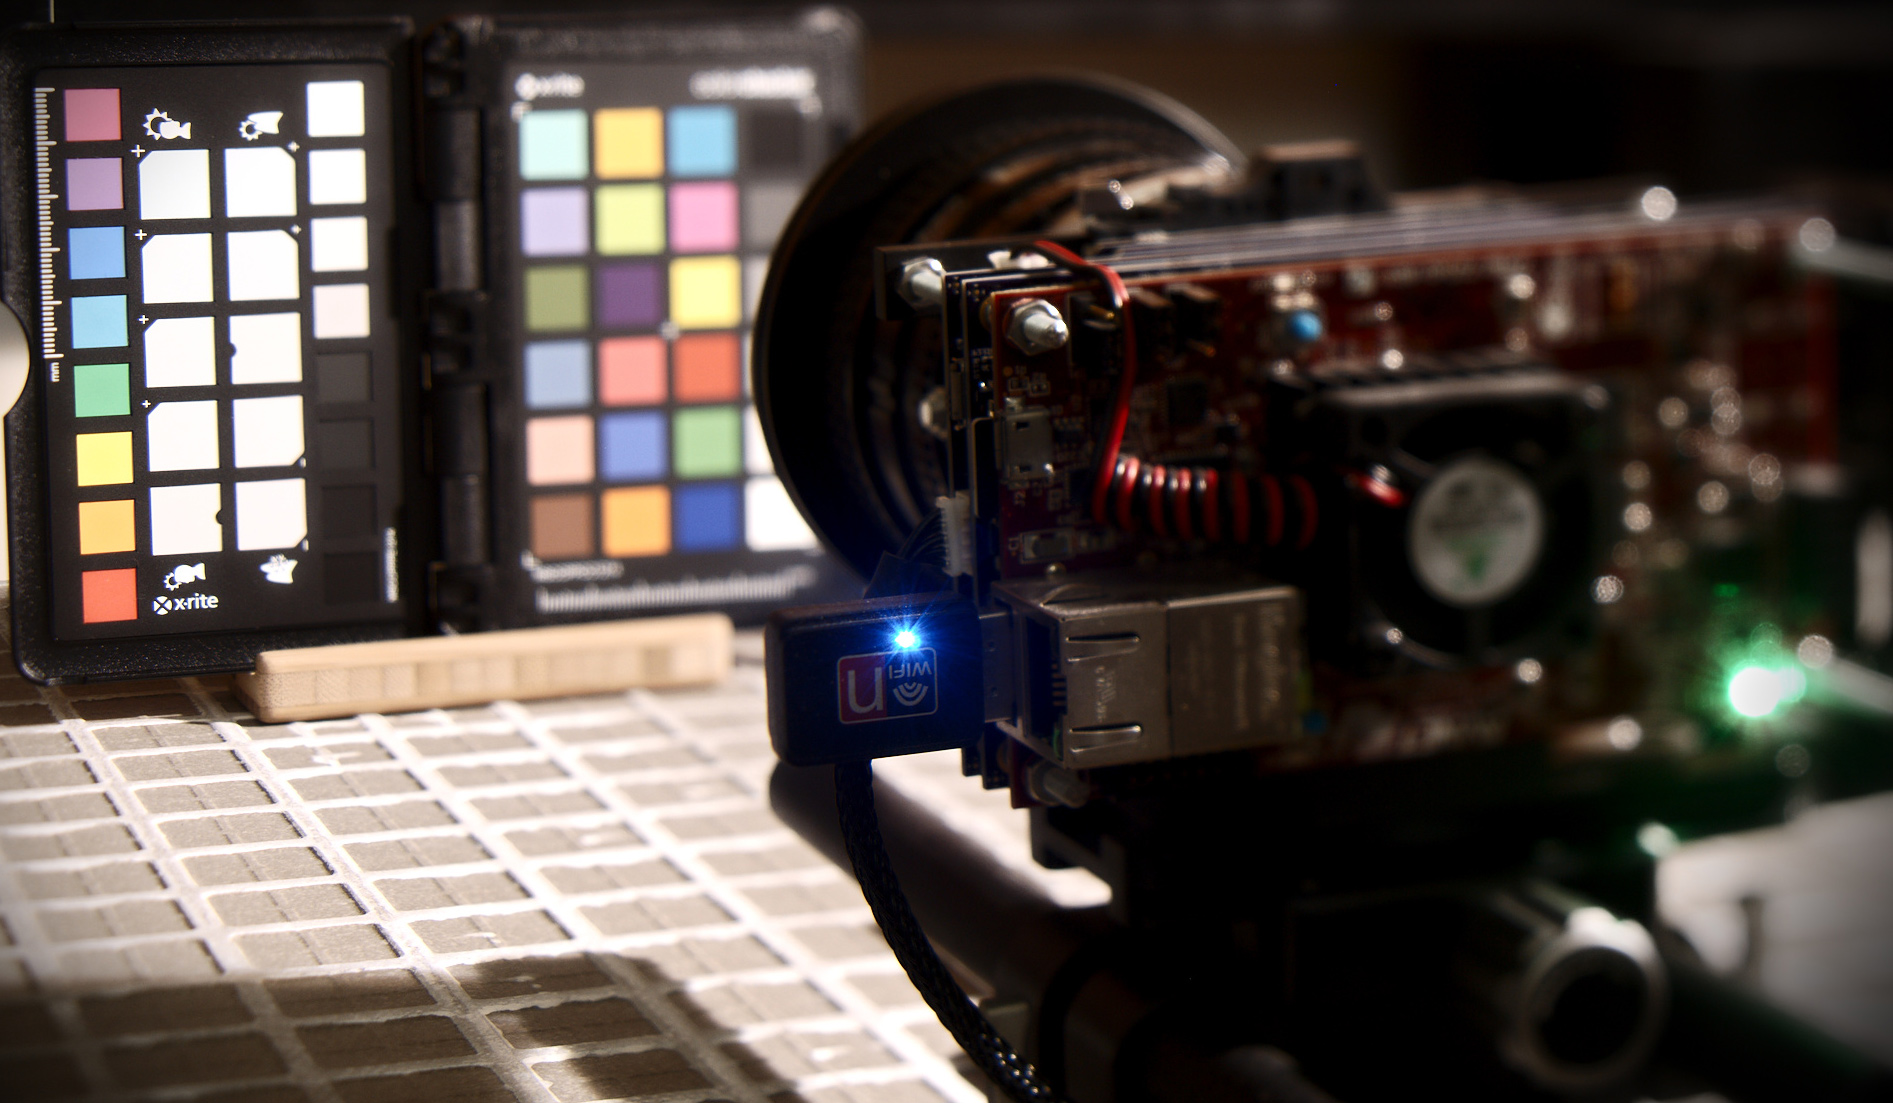
\includegraphics[height=9.6cm]{images/Beta-wifi}\\
\end{center}

Connecting a USB wifi dongle (that supports Soft-AP) to the AXIOM Beta USB port allows controlling the camera via wireless connection.\\

In order to do this you must first check your wifi card: 

\begin{lstlisting}[language=bash,morekeywords=$,keywordstyle=\bfseries,frame=none,xleftmargin=.25in,belowskip=2em, aboveskip=2em]
ifconfig
\end{lstlisting}

Turn on wifi card: 

\begin{lstlisting}[language=bash,morekeywords=$,keywordstyle=\bfseries,frame=none,xleftmargin=.25in,belowskip=2em, aboveskip=2em]
ifconfig wlan0 up
\end{lstlisting}

Search wifi essid/hotspot name: 

\begin{lstlisting}[language=bash,morekeywords=$,keywordstyle=\bfseries,frame=none,xleftmargin=.25in,belowskip=2em, aboveskip=2em]
iwlist wlan0 scan
\end{lstlisting}

Setting up Essid and password:\\

WEP:

\begin{lstlisting}[language=bash,morekeywords=$,keywordstyle=\bfseries,frame=none,xleftmargin=.25in,belowskip=2em, aboveskip=2em]
iwconfig wlan0 essid "yourhotspotname" key yourpassword 
\end{lstlisting}

ASCII:

\begin{lstlisting}[language=bash,morekeywords=$,keywordstyle=\bfseries,frame=none,xleftmargin=.25in,belowskip=2em, aboveskip=2em]
iwconfig wlan0 essid "yourhotspotname" key s:asciikey 
\end{lstlisting}

WPA2 (tested and working) update mirrors database (it is required to connect to the Internet via Ethernet): 

\begin{lstlisting}[language=bash,morekeywords=$,keywordstyle=\bfseries,frame=none,xleftmargin=.25in,belowskip=2em, aboveskip=2em]
pacman -Syy 
\end{lstlisting}

Install wpa\_supplicant: 

\begin{lstlisting}[language=bash,morekeywords=$,keywordstyle=\bfseries,frame=none,xleftmargin=.25in,belowskip=2em, aboveskip=2em]
pacman -S wpa_supplicant
\end{lstlisting}

Configuration with wpa\_passphrase - \href{https://wiki.archlinux.org/index.php/WPA\_supplicant}{https://wiki.archlinux.org/index.php/WPA\_supplicant} create basic configuration file MYSSID = name of your wireless network passphrase = password to connect to your wireless network.

\begin{lstlisting}[language=bash,morekeywords=$,keywordstyle=\bfseries,frame=none,xleftmargin=.25in,belowskip=2em, aboveskip=2em]
wpa_passphrase MYSSID passphrase > /etc/wpa_supplicant/example.conf
\end{lstlisting}

\begin{lstlisting}[language=bash,morekeywords=$,keywordstyle=\bfseries,frame=none,xleftmargin=.25in,belowskip=2em, aboveskip=2em]
ip link set dev wlan0 up
\end{lstlisting}

\begin{lstlisting}[language=bash,morekeywords=$,keywordstyle=\bfseries,frame=none,xleftmargin=.25in,belowskip=2em, aboveskip=2em]
wpa_supplicant -B -i wlan0 -c /etc/wpa_supplicant/example.conf
\end{lstlisting}

If nl80211 driver does not support the given hardware. The deprecated wext driver might still support the device:

\begin{lstlisting}[language=bash,morekeywords=$,keywordstyle=\bfseries,frame=none,xleftmargin=.25in,belowskip=2em, aboveskip=2em]
wpa_supplicant -B -i wlan0 -D wext -c /etc/wpa_supplicant/example.conf
\end{lstlisting}

\begin{lstlisting}[language=bash,morekeywords=$,keywordstyle=\bfseries,frame=none,xleftmargin=.25in,belowskip=2em, aboveskip=2em]
dhcpcd wlan0
\end{lstlisting}

Autostart connect \href{https://wiki.archlinux.org/index.php/netctl}{https://wiki.archlinux.org/index.php/netctl} copy config from example: 

\begin{lstlisting}[language=bash,morekeywords=$,keywordstyle=\bfseries,frame=none,xleftmargin=.25in,belowskip=2em, aboveskip=2em]
cp /etc/netctl/example/wireless-wpa /etc/netctl/wireless-wpa
\end{lstlisting}

Edit the config for you network (interface/ESSID/key): 

\begin{lstlisting}[language=bash,morekeywords=$,keywordstyle=\bfseries,frame=none,xleftmargin=.25in,belowskip=2em, aboveskip=2em]
nano /etc/netctl/wireless-wpa
\end{lstlisting}

First manually check that the profile can be started successfully with: 

\begin{lstlisting}[language=bash,morekeywords=$,keywordstyle=\bfseries,frame=none,xleftmargin=.25in,belowskip=2em, aboveskip=2em]
netctl start wireless-wpa 
\end{lstlisting}

If the above command results in a failure, then use:

\begin{lstlisting}[language=bash,morekeywords=$,keywordstyle=\bfseries,frame=none,xleftmargin=.25in,belowskip=2em, aboveskip=2em]
    journalctl -xn 
    netctl status profile 
\end{lstlisting}

... to obtain a more in depth explanation of the failure. (profile might already been started)\\

Enable: 

\begin{lstlisting}[language=bash,morekeywords=$,keywordstyle=\bfseries,frame=none,xleftmargin=.25in,belowskip=2em, aboveskip=2em]
netctl enable wireless-wpa
\end{lstlisting}

This will create and enable a systemd service that will start when the computer boots. Changes to the profile file will not propagate to the service file automatically. After such changes, it is necessary to reenable the profile: 

\begin{lstlisting}[language=bash,morekeywords=$,keywordstyle=\bfseries,frame=none,xleftmargin=.25in,belowskip=2em, aboveskip=2em]
netctl reenable wireless-wpa
\end{lstlisting}
